
\documentclass{standalone}
\usepackage{xcolor}
\usepackage{pgfplots}
\pgfplotsset{compat=1.18}

\begin{document}

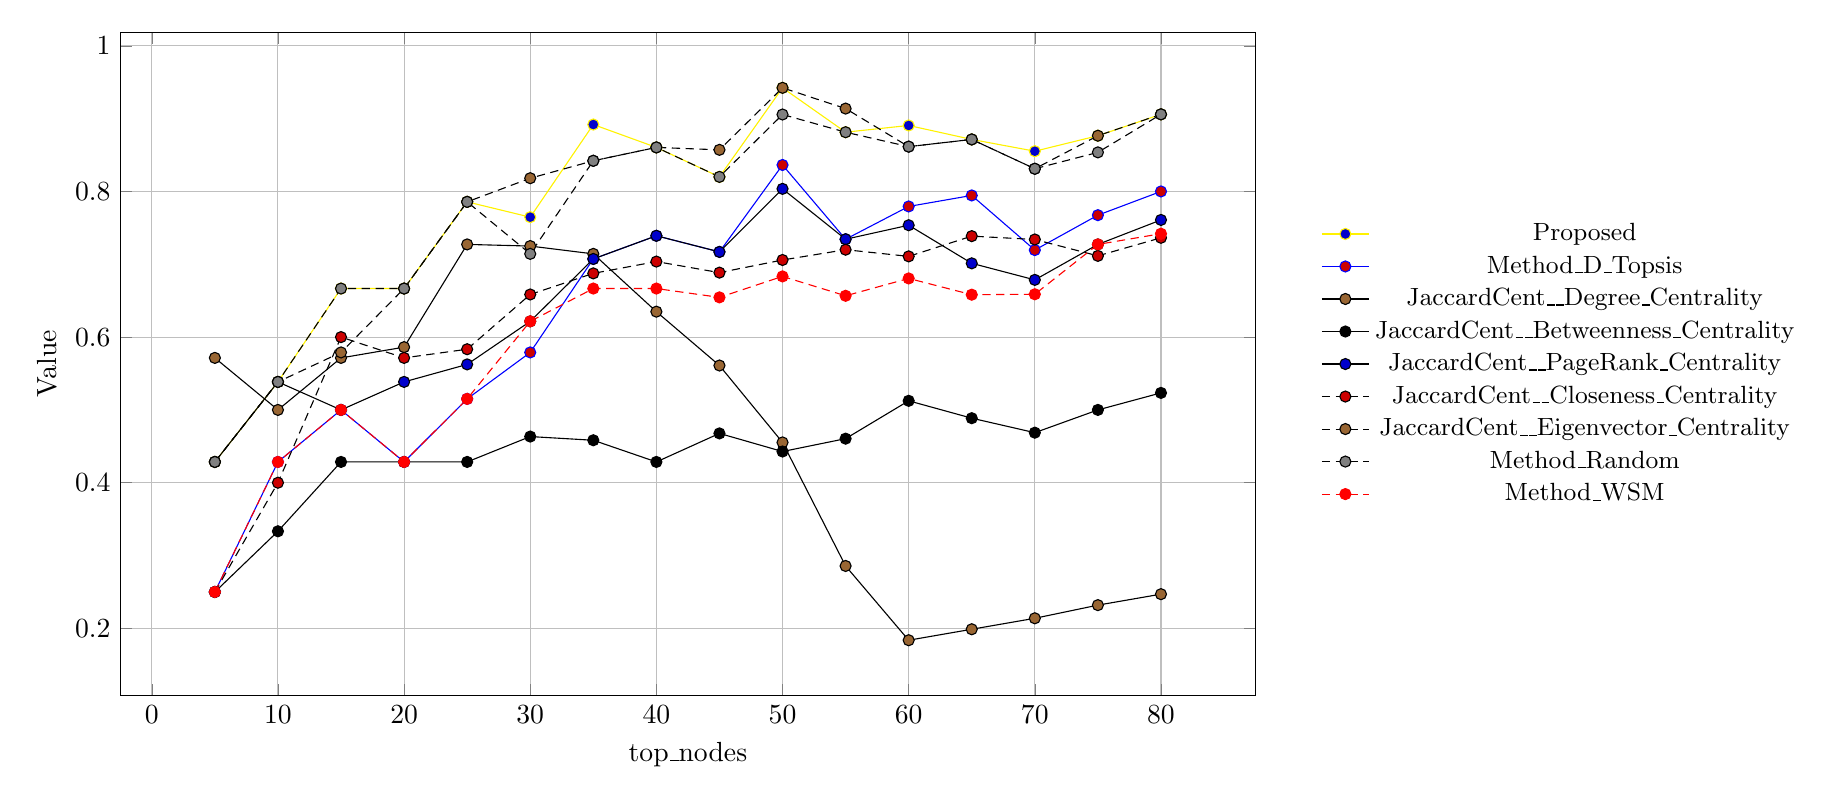
\begin{tikzpicture}
\begin{axis}[
    width=16cm,
    height=10cm,
    xlabel={top\_nodes},
    ylabel={Value},
    grid=major,
    legend style={
        at={(1.05,0.5)},
        anchor=west,
        font=\small,
        draw=none,
        cells={align=left},
    },
]
% Proposed
\addplot+[color=yellow, mark=*] coordinates {
(5.0,0.4285714285714285) (10.0,0.5384615384615384) (15.0,0.6666666666666666) (20.0,0.6666666666666666) (25.0,0.7857142857142857) (30.0,0.7647058823529411) (35.0,0.8918918918918919) (40.0,0.8604651162790697) (45.0,0.82) (50.0,0.9423076923076924) (55.0,0.8813559322033898) (60.0,0.890625) (65.0,0.8714285714285714) (70.0,0.8552631578947368) (75.0,0.8765432098765432) (80.0,0.9058823529411764) };
\addlegendentry{Proposed}

% Method\_D\_Topsis
\addplot+[color=blue, mark=*] coordinates {
(5.0,0.25) (10.0,0.4285714285714285) (15.0,0.5) (20.0,0.4285714285714285) (25.0,0.5151515151515151) (30.0,0.5789473684210527) (35.0,0.7073170731707317) (40.0,0.7391304347826086) (45.0,0.7169811320754716) (50.0,0.8363636363636363) (55.0,0.734375) (60.0,0.7794117647058824) (65.0,0.7945205479452054) (70.0,0.7195121951219512) (75.0,0.7674418604651163) (80.0,0.8) };
\addlegendentry{Method\_D\_Topsis}

% JaccardCent\_\_Degree\_Centrality
\addplot+[color=black, mark=*] coordinates {
(5.0,0.5714285714285714) (10.0,0.5) (15.0,0.5714285714285714) (20.0,0.5862068965517241) (25.0,0.7272727272727273) (30.0,0.725) (35.0,0.7142857142857143) (40.0,0.6349206349206349) (45.0,0.5609756097560976) (50.0,0.4553571428571428) (55.0,0.2857142857142857) (60.0,0.1837349397590361) (65.0,0.1987951807228915) (70.0,0.2138554216867469) (75.0,0.2319277108433735) (80.0,0.2469879518072289) };
\addlegendentry{JaccardCent\_\_Degree\_Centrality}

% JaccardCent\_\_Betweenness\_Centrality
\addplot+[color=black, mark=*] coordinates {
(5.0,0.25) (10.0,0.3333333333333333) (15.0,0.4285714285714285) (20.0,0.4285714285714285) (25.0,0.4285714285714285) (30.0,0.4634146341463415) (35.0,0.4583333333333333) (40.0,0.4285714285714285) (45.0,0.4677419354838709) (50.0,0.4428571428571428) (55.0,0.4605263157894737) (60.0,0.5125) (65.0,0.4886363636363636) (70.0,0.46875) (75.0,0.5) (80.0,0.5233644859813084) };
\addlegendentry{JaccardCent\_\_Betweenness\_Centrality}

% JaccardCent\_\_PageRank\_Centrality
\addplot+[color=black, mark=*] coordinates {
(5.0,0.4285714285714285) (10.0,0.5384615384615384) (15.0,0.5) (20.0,0.5384615384615384) (25.0,0.5625) (30.0,0.6216216216216216) (35.0,0.7073170731707317) (40.0,0.7391304347826086) (45.0,0.7169811320754716) (50.0,0.8035714285714286) (55.0,0.734375) (60.0,0.7536231884057971) (65.0,0.7012987012987013) (70.0,0.6785714285714286) (75.0,0.7272727272727273) (80.0,0.7608695652173914) };
\addlegendentry{JaccardCent\_\_PageRank\_Centrality}

% JaccardCent\_\_Closeness\_Centrality
\addplot+[color=black, mark=*] coordinates {
(5.0,0.25) (10.0,0.4) (15.0,0.6) (20.0,0.5714285714285714) (25.0,0.5833333333333334) (30.0,0.6585365853658537) (35.0,0.6875) (40.0,0.7037037037037037) (45.0,0.6885245901639344) (50.0,0.7058823529411765) (55.0,0.72) (60.0,0.7108433734939759) (65.0,0.7386363636363636) (70.0,0.7340425531914894) (75.0,0.7115384615384616) (80.0,0.7363636363636363) };
\addlegendentry{JaccardCent\_\_Closeness\_Centrality}

% JaccardCent\_\_Eigenvector\_Centrality
\addplot+[color=black, mark=*] coordinates {
(5.0,0.4285714285714285) (10.0,0.5384615384615384) (15.0,0.5789473684210527) (20.0,0.6666666666666666) (25.0,0.7857142857142857) (30.0,0.8181818181818182) (35.0,0.8421052631578947) (40.0,0.8604651162790697) (45.0,0.8571428571428571) (50.0,0.9423076923076924) (55.0,0.913793103448276) (60.0,0.8615384615384616) (65.0,0.8714285714285714) (70.0,0.8311688311688312) (75.0,0.8765432098765432) (80.0,0.9058823529411764) };
\addlegendentry{JaccardCent\_\_Eigenvector\_Centrality}

% Method\_Random
\addplot+[color=black, mark=*] coordinates {
(5.0,0.4285714285714285) (10.0,0.5384615384615384) (15.0,0.6666666666666666) (20.0,0.6666666666666666) (25.0,0.7857142857142857) (30.0,0.7142857142857143) (35.0,0.8421052631578947) (40.0,0.8604651162790697) (45.0,0.82) (50.0,0.9056603773584906) (55.0,0.8813559322033898) (60.0,0.8615384615384616) (65.0,0.8714285714285714) (70.0,0.8311688311688312) (75.0,0.8536585365853658) (80.0,0.9058823529411764) };
\addlegendentry{Method\_Random}

% Method\_WSM
\addplot+[color=red, mark=*] coordinates {
(5.0,0.25) (10.0,0.4285714285714285) (15.0,0.5) (20.0,0.4285714285714285) (25.0,0.5151515151515151) (30.0,0.6216216216216216) (35.0,0.6666666666666666) (40.0,0.6666666666666666) (45.0,0.6545454545454545) (50.0,0.6833333333333333) (55.0,0.6567164179104478) (60.0,0.6805555555555556) (65.0,0.6582278481012658) (70.0,0.6588235294117647) (75.0,0.7272727272727273) (80.0,0.7419354838709677) };
\addlegendentry{Method\_WSM}


\end{axis}
\end{tikzpicture}

\end{document}
